\documentclass{acmconf}
\usepackage{graphicx}
\usepackage{multicol}
\usepackage{amssymb,amsmath,epsfig,alltt}
\sloppy
\usepackage{palatino}
\usepackage{pdftricks}
\begin{psinputs}
  \usepackage{pstricks}
  \usepackage{pst-node}
\end{psinputs}
\usepackage{parskip}
\usepackage{tabularx}
\usepackage{alltt}
\bibliographystyle{amsplain}

\title{\textbf{\textsf{
Complete Translation of Unsafe Native Code to Safe Bytecode
}}}
\date{}
\author{\begin{tabular}{@{}c@{}}
        {\em {Brian Alliet}} \\
        {Rochester Institute of Technology}\\
        {\tt bja8464@cs.rit.edu}
   \end{tabular}\hskip 1in\begin{tabular}{@{}c@{}}
        {\em {Adam Megacz}} \\
        {University of California, Berkeley} \\
        {\tt megacz@cs.berkeley.edu}
\end{tabular}}
\begin{document}

\maketitle

{\it This document was typeset using D. E. Knuth's original \TeX 89,
     which was both compiled and executed entirely within a Java
     Virtual Machine without the use of native code.}

\begin{abstract}

Existing techniques for using code written in an unsafe language
within a safe virtual machine generally involve transformations from
one source code language (such as C, Pascal, or Fortran) to another
(such as Java) which is then compiled into virtual machine bytecodes.

We present an alternative approach which translate MIPS binaries
produced by any compiler into safe virtual machine bytecodes.  This
approach offers four key advantages over existing techniques: it is
language agnostic, it offers bug-for-bug compiler compatability,
requires no post-translation human intervention, and introduces no
build process modifications.

We also present NestedVM, an implementation of this technique, and
discuss its application to six software packages: LINPACK (Fortran),
which was used as one of our performance tests, \TeX\ (Pascal), which
was used to typeset this document, {\tt libjpeg}, {\tt libmspack}, and
FreeType (all C source), which are currently in production use as part
of the Ibex Project, and {\tt gcc}, which was used to compile all of
the aforementioned.

Performance measurements indicate a best case performance within 3x of
native code and worst case typically within 10x, making it an
attractive solution for code which is not performance-critical.

\end{abstract}

\section{Introduction}

Unsafe languages such as C \cite{KR} and C++ \cite{soustroup} have
been in use much longer than any of today's widely accepted safe
languages such as Java \cite{java} and C\# \cite{csharp}.
Consequently, there is a huge library of software written in these
languages.  Although safe languages offer substantial benefits, their
comparatively young age often puts them at a disadvantage when breadth
of existing support code is an important criterion.

The typical solution to this dilemma is to use a native interface such
as JNI \cite{jni} or CNI \cite{cni} to invoke unsafe code from within a
virtual machine or otherwise safe environment.  Unfortunately, there
are a number of situations in which this is not an acceptable
solution.  These situations can be broadly classified into two
categories: {\it security concerns} and {\it portability concerns}.

Security is often a major concern when integrating native code.  Using
Java as an example, JNI and CNI are prohibited in a number of
contexts, including applet environments and servlet containers with a
{\tt SecurityManager}.  Additionally, even in the context of trusted
code, {\tt native} methods invoked via JNI are susceptible to buffer
overflow and heap corruption attacks which are not a concern for
verified, bounds-checked bytecode.

The second class of disadvantages revolves around portability
concerns; native interfaces require the native library to be compiled
ahead of time for every architecture on which it will be deployed.
This is unacceptable for scenarios in which the full set of target
architectures is not known at deployment time.  Additionally, some JVM
platform variants such as J2ME \cite{j2me} simply do not offer support
for native code.

The technique we present here uses typical compiler to compile unsafe
code into a MIPS binary, which is then translated on an
instruction-by-instruction basis into Java bytecode.  The technique
presented here is general; we anticipate that it can be applied to
other secure virtual machines such as Microsoft's .NET \cite{msil},
Perl Parrot \cite{parrot}, or Python bytecode \cite{python}.

The remainder of this paper is divided as follows: in the next section
we review the relevant set of program representations (safe source,
unsafe source, binary, and bytecode) and survey existing work for
performing transformations between them.  In the third section we
introduce NestedVM and cover its two primary translation modes in
detail.  Section four adresses the optimizations we employ and
quantifies NestedVM's performance.  Section five describes the
NestedVM runtime, which plays the role of the OS kernel.  We conclude
with an analysis of NestedVM's weaknesses and potential for future
improvements.


\section{Approaches to Translation}

The four program representations of interest in this context, along
with their specific types in the C-to-JVM instantiation of the
problem are shown in the following diagram:

\begin{pdfpic}
\newlength{\MyLength}
\settowidth{\MyLength}{machine code}
\newcommand{\MyBox}[1]{\makebox[\MyLength][c]{#1}}
\begin{psmatrix}[colsep=2,rowsep=0]
  & \\[0pt]
  [name=s0]\MyBox{unsafe source} & [name=s1]\MyBox{safe source}   \\[0pt]
  [name=s00]\MyBox{\tt (.c)} & [name=s11]\MyBox{\tt (.java)}   \\[0pt]
  & \\[0pt]
  & \\[0pt]
  & \\[0pt]
  [name=b0]\MyBox{machine code}  & [name=b1]\MyBox{safe bytecode} \\[0pt]
  [name=b00]\MyBox{\tt (.o)}  & [name=b11]\MyBox{\tt (.class)} \\
  & \\[0pt]
  \psset{nodesep=5pt,arrows=->}
\end{psmatrix}
\end{pdfpic}

To illustrate the context of this diagram, the following arcs show the
translations performed by a few familiar tools:

\begin{pdfpic}
\newlength{\MyLength}
\settowidth{\MyLength}{xmachine codex}
\newcommand{\MyBox}[1]{\makebox[\MyLength]{#1}}
\psmatrix[colsep=2,rowsep=0,nrot=:D]
  & \\[0pt]
  [name=s0]\MyBox{unsafe source} & [name=s1]\MyBox{safe source}   \\[0pt]
  & \\[0pt]
  & \\[0pt]
  & \\[0pt]
  & \\[0pt]
  & \\[0pt]
  [name=b0]\MyBox{machine code}  & [name=b1]\MyBox{safe bytecode} \\[0pt]
  & \\[0pt]
  \psset{nodesep=5pt,arrows=->}
  \ncline{s0}{b0}\bput{:U}{\tt gcc}
  \ncline{s1}{b0}\bput{:D}{\tt gcj}
  \ncline{s1}{b1}\aput{:U}{\tt javac}
  \ncline{b1}{b0}\aput{:D}{\tt gcj}\bput{:D}{JITs}
\endpsmatrix
\end{pdfpic}

Existing techniques for translating unsafe code into VM bytecode
generally fall into two categories, which we expand upon in the
remainder of this section: source-to-source translation and
source-to-binary translation.

\subsection{Source-to-Source Translation}

The most common technique employed is partial translation from unsafe
source code to safe source code:

\begin{pdfpic}
\newlength{\MyLength}
\settowidth{\MyLength}{xmachine codex}
\newcommand{\MyBox}[1]{\makebox[\MyLength]{#1}}
\psmatrix[colsep=2,rowsep=0,nrot=:U]
  & \\[0pt]
  & \\[0pt]
  [name=s0]\MyBox{unsafe source} & [name=s1]\MyBox{safe source}   \\[0pt]
  & \\[0pt]
  & \\[0pt]
  & \\[0pt]
  & \\[0pt]
  & \\[0pt]
  [name=b0]\MyBox{machine code}  & [name=b1]\MyBox{safe bytecode} \\[0pt]
  & \\[0pt]
  \psset{nodesep=5pt,arrows=->}
  \ncline{s0}{s1}\aput{:U}{source-to}\bput{:U}{source}
  \ncline{s1}{b1}\aput{:U}{\tt javac}
\endpsmatrix
\end{pdfpic}

A number of existing systems employ this technique; they can
be divided into two categories: those which perform a partial
translation which is completed by a human, and those which perform a
total translation but fail (yield an error) on a large class of input
programs.


Jazillian \cite{jazillian} is a commercial solution which produces
extremely readable Java source code from C source code, but ony
translates a small portion of the C language.  Jazillian is unique in
that in addition to {\it language migration}, it also performs {\it
API migration}; for example, Jazillian is intelligent enough
to translate {\tt char*~s1~=~strcpy(s2)} into {\tt String~s1~=~s2}.

Unfortunately such deep analysis is intractible for most of the C
language and standard library; Jazillian's documentation notes that
{\it ``This is not your father's language translator.  It's not
generating ugly code that's guaranteed to work out of the
box... Jazillian does not always produce code that works correctly.''}

MoHCA-Java \cite{mohca} is the other major tool in this category, and steps
beyond Jazillian by providing tools for analysis of the source C++
abstract syntax tree.  Additionally, MoHCA-Java's analysis engine is
extensible, making it a platform for constructing application-specific
translators rather than a single translation tool.  However,
MoHCA-Java does not always generate complete Java code for all of the C++
programs which it accepts.

The c2j \cite{c2j}, c2j++ \cite{c2jpp}, Cappucinno \cite{capp},
and Ephedra \cite{ephedra} systems each provide support for complete
translation of a {\it subset} of the source language (C or C++).  Each
of the four tools supports a progressively greater subset than the one
preceding it; however none covers the entire input language.

Ephedra, the most advanced of the four, supports most of the C++
language, and claims to produce ``human readable'' Java code as
output.  Notable omissions from the input domain include support for
fully general pointer arithmetic, casting between unrelated types, and
reading from a {\tt union} via a different member than the one most
recently written.

Unfortunately, when the program being translated is large and complex,
it is quite likely that it will use an unsupported feature in at least
one place.  In the absence of a programmer who understands the source
program, a single anomoly is often enough to render the entire
translation process useless.  As a result, these tools are mainly
useful as an {\it aid} to programmers who could normally perform the
conversion themselves, but want to save time by automating most of the
process.


\subsection{Source-to-Binary Translation}

Source-to-binary translation involves a compiler for the unsafe
language which has been modified to emit safe bytecode.

\begin{pdfpic}
\newlength{\MyLength}
\settowidth{\MyLength}{xmachine codex}
\newcommand{\MyBox}[1]{\makebox[\MyLength]{#1}}
\psmatrix[colsep=2,rowsep=0,nrot=:U]
  & \\[0pt]
  [name=s0]\MyBox{unsafe source} & [name=s1]\MyBox{safe source}   \\[0pt]
  & \\[0pt]
  & \\[0pt]
  & \\[0pt]
  & \\[0pt]
  & \\[0pt]
  [name=b0]\MyBox{machine code}  & [name=b1]\MyBox{safe bytecode} \\[0pt]
  & \\[0pt]
  \psset{nodesep=5pt,arrows=->}
  \ncline{s0}{b1}\bput{:U}{source-to-binary}
\endpsmatrix
\end{pdfpic}

The primary occupant of this category is {\tt egcs-jvm}
\cite{egcsjvm}, an experimental ``JVM backend'' for the GNU Compiler
Collection ( {\tt gcc} ) \cite{gcc}.  Since {\tt gcc} employs a highly
modular architecture, it {\it is} possible to add RTL code generators
for nonstandard processors.  However, {\tt gcc}'s parsing, RTL
generation, and optimization layers make fundamental assumptions (such
as the availability of pointer math) which cannot be directly
supported; thus the compiler still fails for a substantial class of
input programs.

A Java backend for the {\tt lcc} [CITE] compiler, known as {\tt
lcc-java} [CITE], but was not completed.  {\tt lcc-java} also lacks
any form of system library ({\tt libc}), so very few C programs will
run without custom modification, which would cause them to diverge
from the upstream sources.  Finally, {\tt lcc-java}'s memory model is
much more restricted; it uses a fixed-size array to represent all
memory, and expands the array by allocating a new array and copying,
which is extremely inefficient.  No attempt is made to take advantage
of {\tt NullPointerException} checking (which costs nothing if the
exception is not thrown since most JVMs use the MMU to detect this).
Finally, {\tt lcc-java} targets Java source code, which places the
vast majority of NestedVM's optimizations beyond its reach, and
severely restricts the maximum program size {\tt lcc-java} can handle.

Finally, {\tt lcc-java} maintains a separate memory area for the
stack, which appears to limit the exchange of stack pointers and heap
pointers.  It is unclear from the documentation how this is handled.


\section{NestedVM}

The principal difference between NestedVM and other approaches is that
NestedVM {\it does not} attempt to deal with source code as an input,
instead opting for {\it binary-to-source} and {\it binary-to-binary}
translation.  This offers three immediate advantages:

\begin{itemize}
\item {\bf Language Agnostic}

      Because NestedVM does not attempt to implement the parsing and
      code generation steps of compilation, it is freed from the
      extremely complex task of faithfully implementing languages
      which are often not fully or formally specified (such as C and
      C++), and is able to support any langage for which a
      MIPS-targeted compiler exists.

\item {\bf Bug-for-bug compiler compatability}

      Since NestedVM uses the compiler's {\it output} as its own {\it
      input}, it ensures that programs which are inadvertently
      dependent on the vagaries of a particular compiler can still be
      used.

\item {\bf No build process modifications}

      NestedVM does not modify existing build processes, which can be
      extremely complex and dependent on strange preprocessor usage as
      well as the complex interplay between compiler switches and
      header file locations.

\end{itemize}

NestedVM's approach carries a fourth benefit as well, arising from its
totality:

\begin{itemize}
\item {\bf No post-translation human intervention}

      NestedVM offers total support for all non-privileged
      instructions, registers, and resources found on a MIPS {\tt
      R2000} CPU, including the add/multiply unit and floating point
      coprocessor.  As such, it constitutes a total function mapping
      from the entire domain of (non-kernel-mode) programs onto (a
      subset of) the semantics of the Java Virtual Machine.  This
      ensures that the translation process is fully automated and
      always succeeds for valid input binaries.
\end{itemize}

This is a much more important factor than is obvious at first glance.
If post-translation human intervention is required, then the {\it
human becomes part of the build process}.  This means that if a third
party library used in the project needs to be upgraded, {\it a human
must intervene} in the rebuild process.  In addition to slowing the
process and introducing opportunities for error, this task often
requires specialized knowledge which becomes tied to the particular
individual performing this task, rather than being encoded in build
scripts which persist throughout the lifetime of the project.

\subsection{Why MIPS?}

We chose MIPS as a source format for three reasons: the availability
of tools to compile legacy code into MIPS binaries, the close
similarity (FIXME: explain) between the MIPS ISA and the Java Virtual
Machine, and the relatively high degree of program structure that can
be inferred from ABI-adherent binaries.

The MIPS architecture has been around for quite some time, and is well
supported by the GNU Compiler Collection, which is capable of
compiling C, C++, Java, Fortran, Pascal, and Objective C
into MIPS binaries.

The MIPS R2000 ISA bears a striking similarity to the Java Virtual
Machine:

\begin{itemize}

\item Most of the instructions in the original MIPS ISA operate only
      on 32-bit aligned memory locations. This allows NestedVM to
      represent memory as a Java {\tt int[]} array without introducing
      additional overhead.  The remaining non-aligned memory load
      instructions are only rarely emitted by most compilers since
      they carry a performance penalty on physical MIPS
      implementations.

\item Unlike its predecessor, the R2000 supports 32-bit by 32-bit
      multiply and divide instructions as well as a single and double
      precision floating point unit.  These capabilities map nicely
      onto Java's arithmetic instructions.

\item Although MIPS offers unsigned arithmetic and Java does not, few
      MIPS instructions actually depend on non-two's-complement
      handling of integer math.  Furthermore, since most high-level
      languages such as C do not expose access to arithmetic-overflow
      exceptions, these instructions are rarely found except in
      hand-coded assembler.  In the few situations where these
      instructions {\it are} encountered, the {\tt unsigned int} is
      cast (bitwise) to a Java {\tt long}, the operation is performed,
      and the result is cast back.  On architectures offering 64-bit
      integer math this conversion carries no overhead.
      
\end{itemize}

Finally, the MIPS ISA and ABI convey quite a bit of information about
program structure.  This information can be used for optimization
purposes:

\begin{itemize}

\item The structure of MIPS branching and jump instructions make it
      easy to infer the set of likely target instructions.

\item The MIPS ABI specifies particular registers as caller-save and
      callee-save, as well as designating a register for the return
      address after a function call.  This allows NestedVM to optimize
      many operations for the common case of ABI-adherent binaries.

\item All MIPS instructions are exactly 32 bits long.

\end{itemize}



\subsection{Binary-to-Source}

The simplest operational mode for NestedVM is binary-to-source
translation.  In this mode, NestedVM translates MIPS binaries into
Java source code, which is then fed to a Java compiler in order to
produce bytecode files:

\begin{pdfpic}
\newlength{\MyLength}
\settowidth{\MyLength}{xmachine codex}
\newcommand{\MyBox}[1]{\makebox[\MyLength]{#1}}
\psmatrix[colsep=2,rowsep=0,nrot=:U]
  & \\[0pt]
  & \\[0pt]
  [name=s0]\MyBox{unsafe source} & [name=s1]\MyBox{safe source}   \\[0pt]
  & \\[0pt]
  & \\[0pt]
  & \\[0pt]
  & \\[0pt]
  & \\[0pt]
  [name=b0]\MyBox{machine code}  & [name=b1]\MyBox{safe bytecode} \\[0pt]
  \psset{nodesep=5pt,arrows=->}
  \ncline{s0}{b0}\bput{:U}{\tt gcc}
  \ncline{s1}{b1}\aput{:U}{\tt javac}
  \ncline{b0}{s1}\naput{\tt NestedVM}
\endpsmatrix
\end{pdfpic}

\begin{figure*}[t]
\begin{minipage}[c]{7in}%
\begin{multicols}{2}
{\footnotesize\begin{verbatim}
private final static int r0 = 0;
private int r1, r2, r3,...,r30;
private int r31 = 0xdeadbeef;
private int pc = ENTRY_POINT;

public void run() {
    for(;;) {
        switch(pc) {
            case 0x10000:
                r29 = r29 - 32;
            case 0x10004:
                r1 = r4 + r5;
            case 0x10008:
                if(r1 == r6) {
                    /* delay slot */
                    r1 = r1 + 1;
                    pc = 0x10018:
                    continue;
                }
            case 0x1000C:
                r1 = r1 + 1;
            case 0x10010:
                r31 = 0x10018;
                pc = 0x10210;
                continue;
            case 0x10014:
                /* nop */
            case 0x10018:
                pc = r31;
                continue;
            ...
            case 0xdeadbeef:
                System.err.println(``Exited.'');
                System.exit(1);
        }
    }
}
\end{verbatim}}
\vspace{1in}
{\footnotesize\begin{verbatim}
public void run_0x10000() {
    for(;;) {
    switch(pc) {
        case 0x10000:
            ...
        case 0x10004:
            ...
        ...
        case 0x10010:
            r31 = 0x10018;
            pc = 0x10210;
            return;
        ...
    }
    }
}

pubic void run_0x10200() {
    for(;;) {
    switch(pc) {
        case 0x10200:
            ...
        case 0x10204:
            ...
    }
    }
}

public void trampoline() {
    for(;;) {
    switch(pc&0xfffffe00) {
            case 0x10000: run_0x10000(); break;
            case 0x10200: run_0x10200(); break;
            case 0xdeadbe00:
                ...
        }
    }
}
\end{verbatim}}
\end{multicols}
\end{minipage}
\caption{\label{code1} Trampoline transformation necessitated by Java's 64kb method size limit}
\end{figure*}

Translating unsafe code for use within a JVM proceeds as follows:

\begin{enumerate}

\item Compile the source code to a statically linked binary, targeting
      the MIPS R2000 ISA.  Typically this will involve linking against
      {\tt libc}, which translates system requests (such as {\tt
      open()}, {\tt read()}, or {\tt write()}) into appropriate
      invocations of the MIPS {\tt SYSCALL} instruction.  Any other
      libraries which are not tied to a particular OS kernel can be
      linked in (even in binary form) using standard linker commands.
      
\item Invoke {\tt NestedVM} on the statically linked binary.

\item Compile the resulting {\tt .java} code using {\tt jikes}
      \cite{jikes} or {\tt javac}.

\item From java code, invoke the {\tt run()} method on the generated
      class.  This is equivalent to the {\tt main()} entry point.

\end{enumerate}


\subsection{Binary-to-Binary}

After implementing the binary-to-source compiler, a binary-to-binary
translation mode was added.

\begin{pdfpic}
\newlength{\MyLength}
\settowidth{\MyLength}{xmachine codex}
\newcommand{\MyBox}[1]{\makebox[\MyLength]{#1}}
\psmatrix[colsep=2,rowsep=0,nrot=:U]
  & \\[0pt]
  [name=s0]\MyBox{unsafe source} & [name=s1]\MyBox{safe source}   \\[0pt]
  & \\[0pt]
  & \\[0pt]
  & \\[0pt]
  & \\[0pt]
  & \\[0pt]
  [name=b0]\MyBox{machine code}  & [name=b1]\MyBox{safe bytecode} \\[0pt]
  & \\[0pt]
  \psset{nodesep=5pt,arrows=->}
  \ncline{s0}{b0}\bput{:U}{\tt gcc}
  \ncline{b0}{b1}\naput{\tt NestedVM}
\endpsmatrix
\end{pdfpic}

This mode has several advantages:

\begin{itemize}
      
\item There are quite a few interesting bytecode sequences that cannot
      be generated as a result of compiling Java source code.

\item Directly generating {\tt .class} files Eliminates the
      time-consuming {\tt javac} step.

\item Direct compilation to {\tt .class} files opens up the
      interesting possibility of dynamically translating MIPS binaries
      and loading them via {\tt ClassLoader.fromBytes()} {\it at
      deployment time}, eliminating the need to compile binaries ahead
      of time.

\end{itemize}

\section{Optimization and Quantitative Performance}

\subsection{Binary-to-Source mode}

Generating Java source code instead of bytecode frees NestedVM from
having to perform simple constant propagation optimizations, as most
Java compilers already do this.  A recurring example is the treatment
of the {\tt r0} register, which is fixed as {\tt 0} in the MIPS ISA.

Lacking the ability to generate specially optimized bytecode
sequences, a straightforward mapping of the general purpose hardware
registers to 32 {\tt int} fields turned out to be optimal.


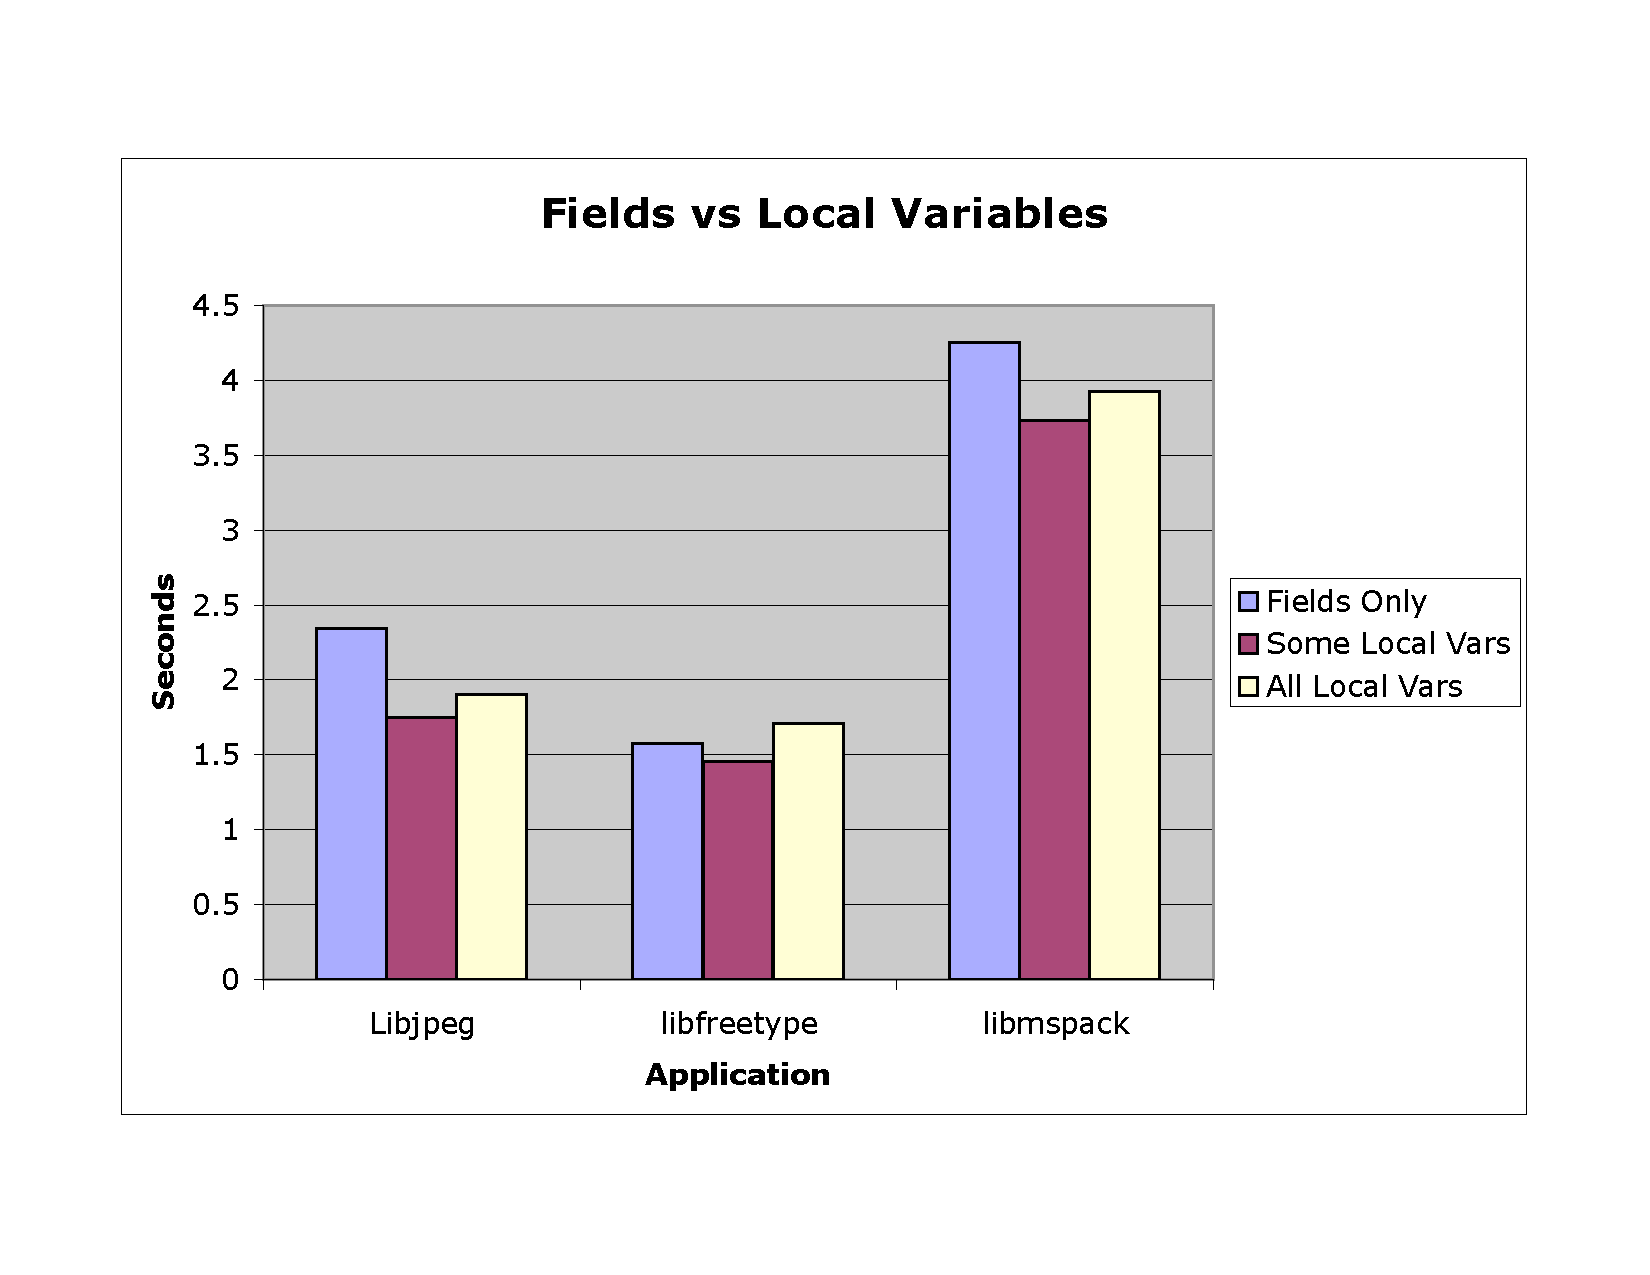
\epsfig{file=charts/chart1,width=3in}

Unfortunately, Java imposes a 64kb limit on the size of the bytecode
for a single method.  This presents a problem for NestedVM, and
necessitates a {\it trampoline transformation}, as shown in
Figure~\ref{code1}.  With this trampoline in place, large binaries can
be handled without much difficulty -- fortunately, there is no
corresponding limit on the size of a classfile as a whole.

One difficulty that arose as a result of using the trampoline
transformation was the fact that {\tt javac} and {\tt jikes} are
unable to properly optimize its switch statements.  For example, the
following code is compiled into a comparatively inefficient {\tt
LOOKUPSWITCH}:

{\footnotesize
\begin{verbatim}
    switch(pc&0xffffff00) {
        case 0x00000100: run_100(); break;
        case 0x00000200: run_200(); break;
        case 0x00000300: run_300(); break;
    }
\end{verbatim}}

Whereas the next block of code code optimized into a {\tt
TABLESWITCH}:

{\footnotesize
\begin{verbatim}
    switch(pc>>>8) {
        case 0x1: run_100();
        case 0x2: run_200();
        case 0x3: run_300();
    }
\end{verbatim}}

This problem was surmounted by switching on a denser set of {\tt case}
values, which is more amenable to the {\tt TABLESWITCH} structure.
This change alone nearly doubled the speed of the compiled binary.

The next performance improvement came from tuning the size of the
methods invoked from the trampoline.  Trial and error led to the
onclusion that HotSpot \cite{hotspot} -- the most widely deployed JVM
-- performs best when 128 MIPS instructions are mapped to each method.

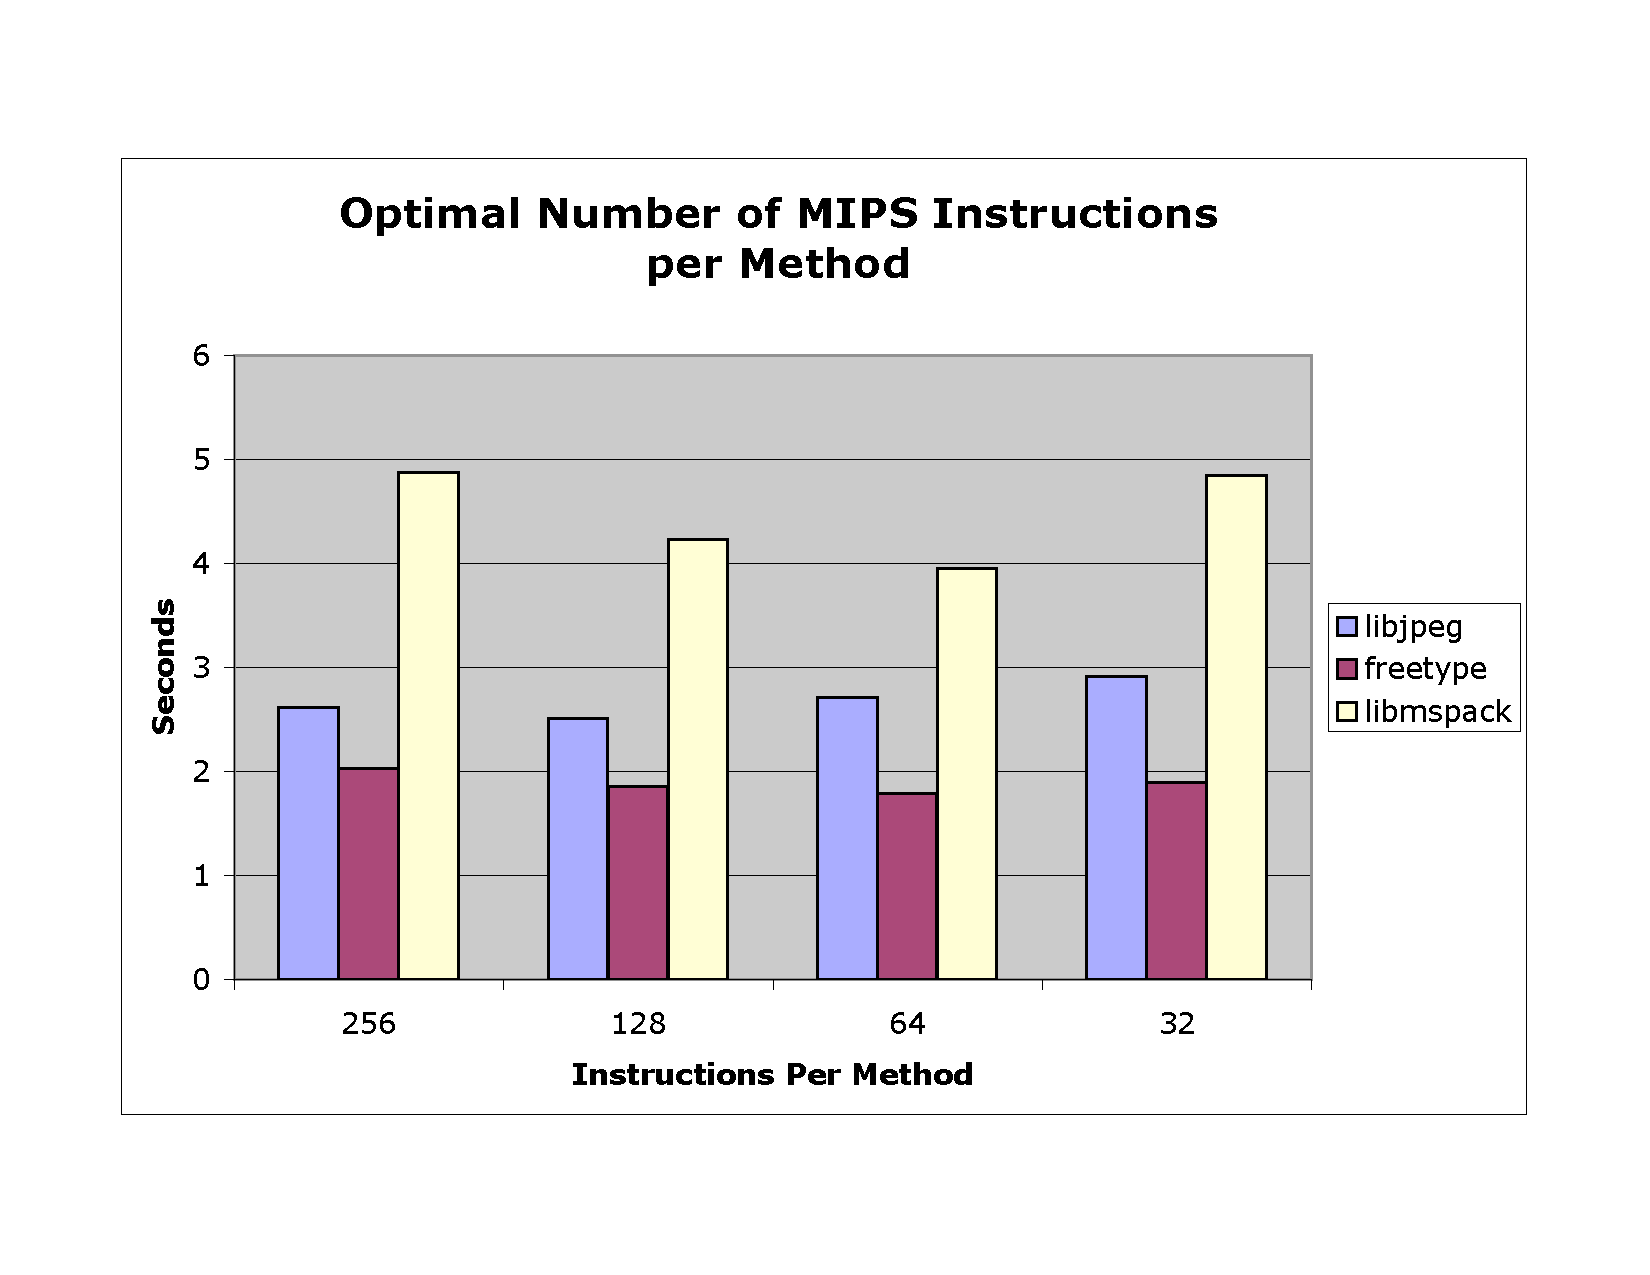
\epsfig{file=chart5,width=3in}

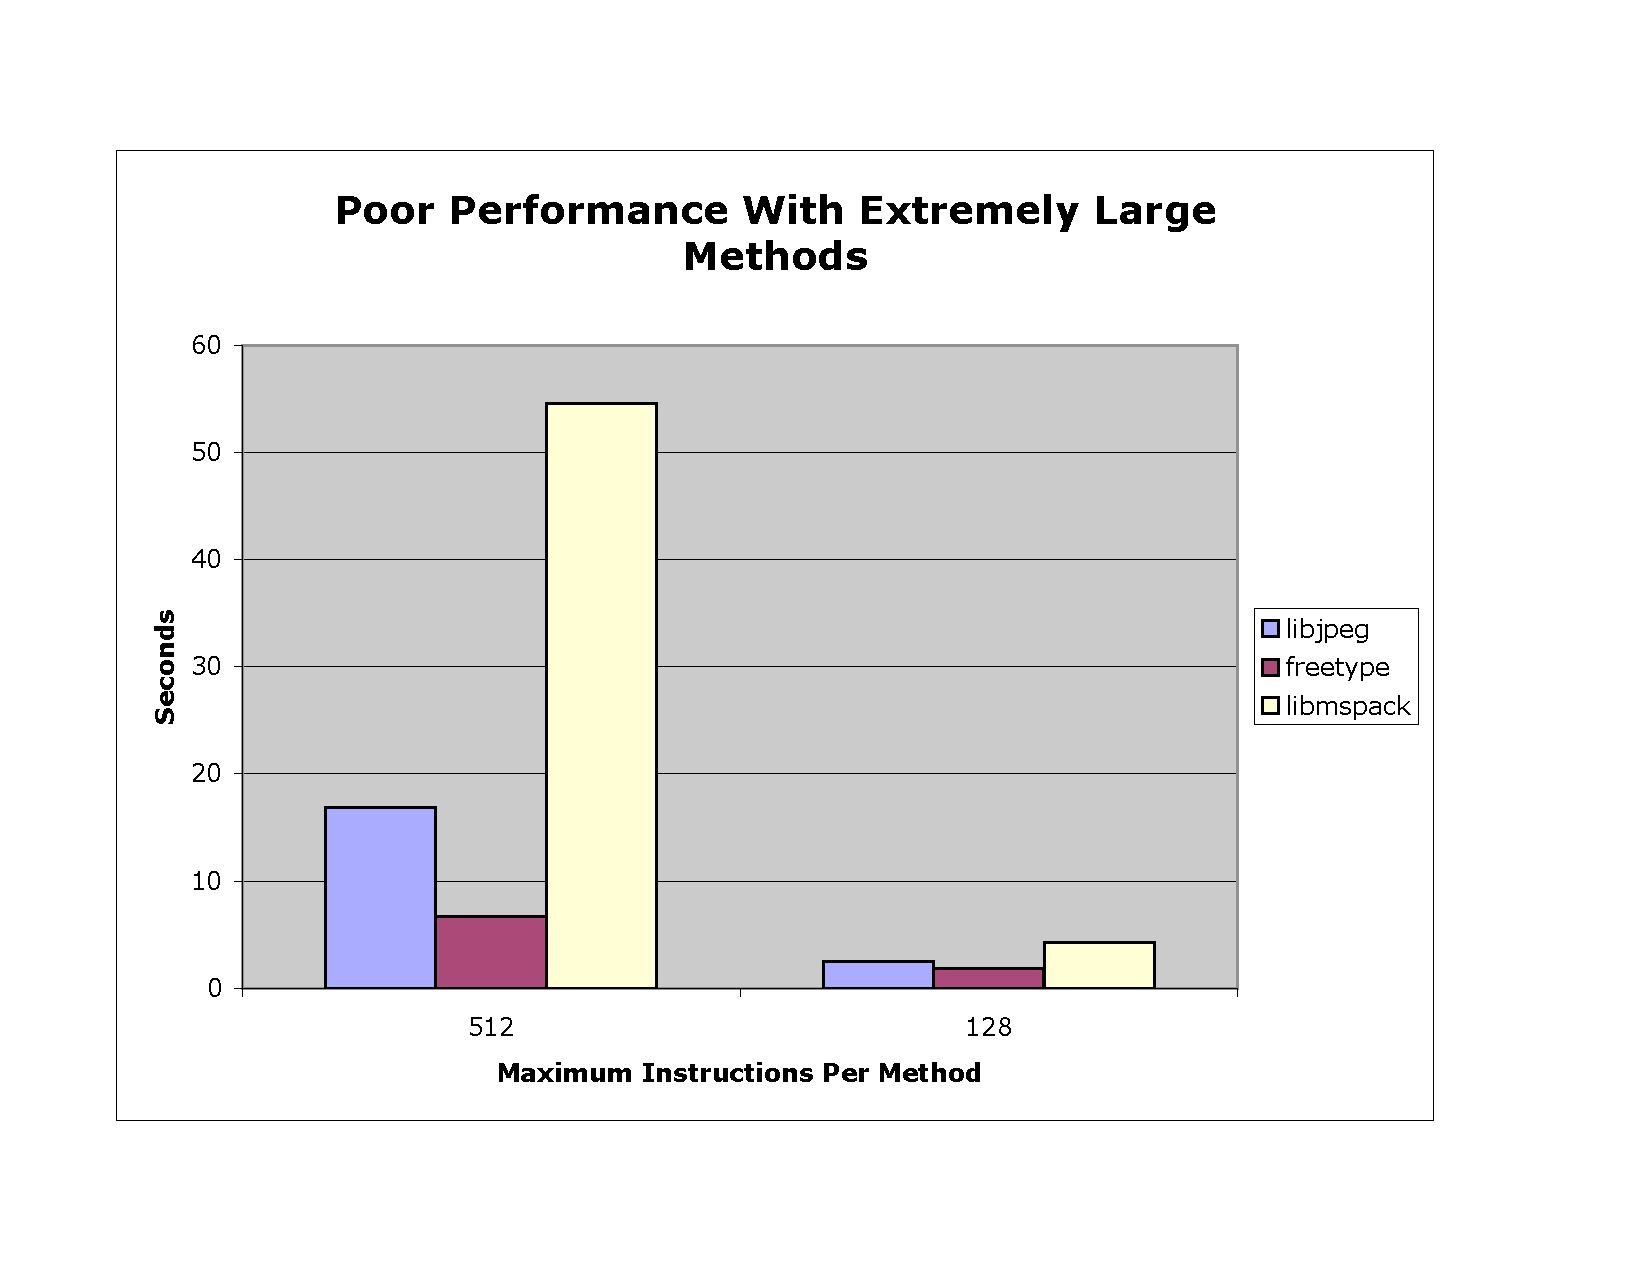
\epsfig{file=chart6,width=3in}

This phenomenon is due to two factors:

\begin{itemize}

\item While the trampoline method's {\tt switch} statement can be
      coded as a {\tt TABLESWITCH}, the {\tt switch} statement
      within the individual methods is to sparse to encode this way.

\item Hybrid Interpretive-JIT compilers such as HotSpot generally
      favor smaller methods since they are easier to compile and are
      better candidates for compilation in ``normal'' programs (unlike
      NestedVM programs).

\end{itemize}

After tuning method sizes, our next performance boost came from
eliminating exraneous case branches.  Having case statements before
each instruction prevents JIT compilers from being able to optimize
across instruction boundaries, since control flow can enter the body
of a {\tt switch} statement at any of the {\tt case}s.  In order to
eliminate unnecessary case statements we needed to identify all
possible jump targets.  Jump targets can come from three sources:

\begin{itemize}

\item {\bf The {\tt .text} segment}

      Every instruction in the text segment is scanned, and every
      branch instruction's destination is added to the list of
      possible branch targets.  In addition, any function that sets
      the link register is added to the list \footnote{actually {\tt addr+8}}.
      Finally, combinations of {\tt LUI} (Load Upper Immediate) and
      {\tt ADDIU} (Add Immediate Unsigned) are scanned for possible
      addresses in the {\tt .text} segment since this combination of
      instructions is often used to load a 32-bit word into a
      register.

\item {\bf The {\tt .data} segment}

      When compiling {\tt switch} statements, compilers often use a
      jump table stored in the {\tt .data} segment.  Unfortunately
      they typically do not identify these jump tables in any way.
      Therefore, the entire {\tt .data} segment is conservatively
      scanned for possible addresses in the {\tt .text} segment.
      
\item {\bf The symbol table}

      This is mainly used as a backup.  Scanning the {\tt .text} and
      {\tt .data} segments should identify any possible jump targets;
      however, adding all function symbols in the ELF symbol table
      also catches functions that are never called directly from the
      MIPS binary, such as those invoked only via the NestedVM
      runtime's {\tt call()} method.

\end{itemize}

Eliminating unnecessary {\tt case} statements provided a 10-25\% speed
increase.

Despite all the above optimizations, one insurmountable obstacle
remained: the Java {\tt .class} file format limits the constant pool
to 65535 entries.  Every integer literal greater than {\tt 32767}
requires an entry in this pool, and each branch instruction generates
one of these.

One suboptimal solution was to express constants as offsets from a few
central values; for example ``{\tt pc~=~N\_0x00010000~+~0x10}'' (where
{\tt N\_0x000100000} is a non-final field to prevent {\tt javac} from
inlining it).  This was sufficient to get reasonably large binaries to
compile, and caused only a small (approximately 5\%) performance
degredation and a similarly small increase in the size of the {\tt
.class} file.  However, as we will see in the next section, compiling
directly to {\tt .class} files (without the intermediate {\tt .java}
file) eliminates this problem entirely.

\subsection{Binary-to-Binary mode}

Most of the performance improvemen where made where in the handling of
branch instructions and in taking advantage of the JVM stack to
eliminate unnecessary {\tt LOAD}s and {\tt STORE}s to local variables.

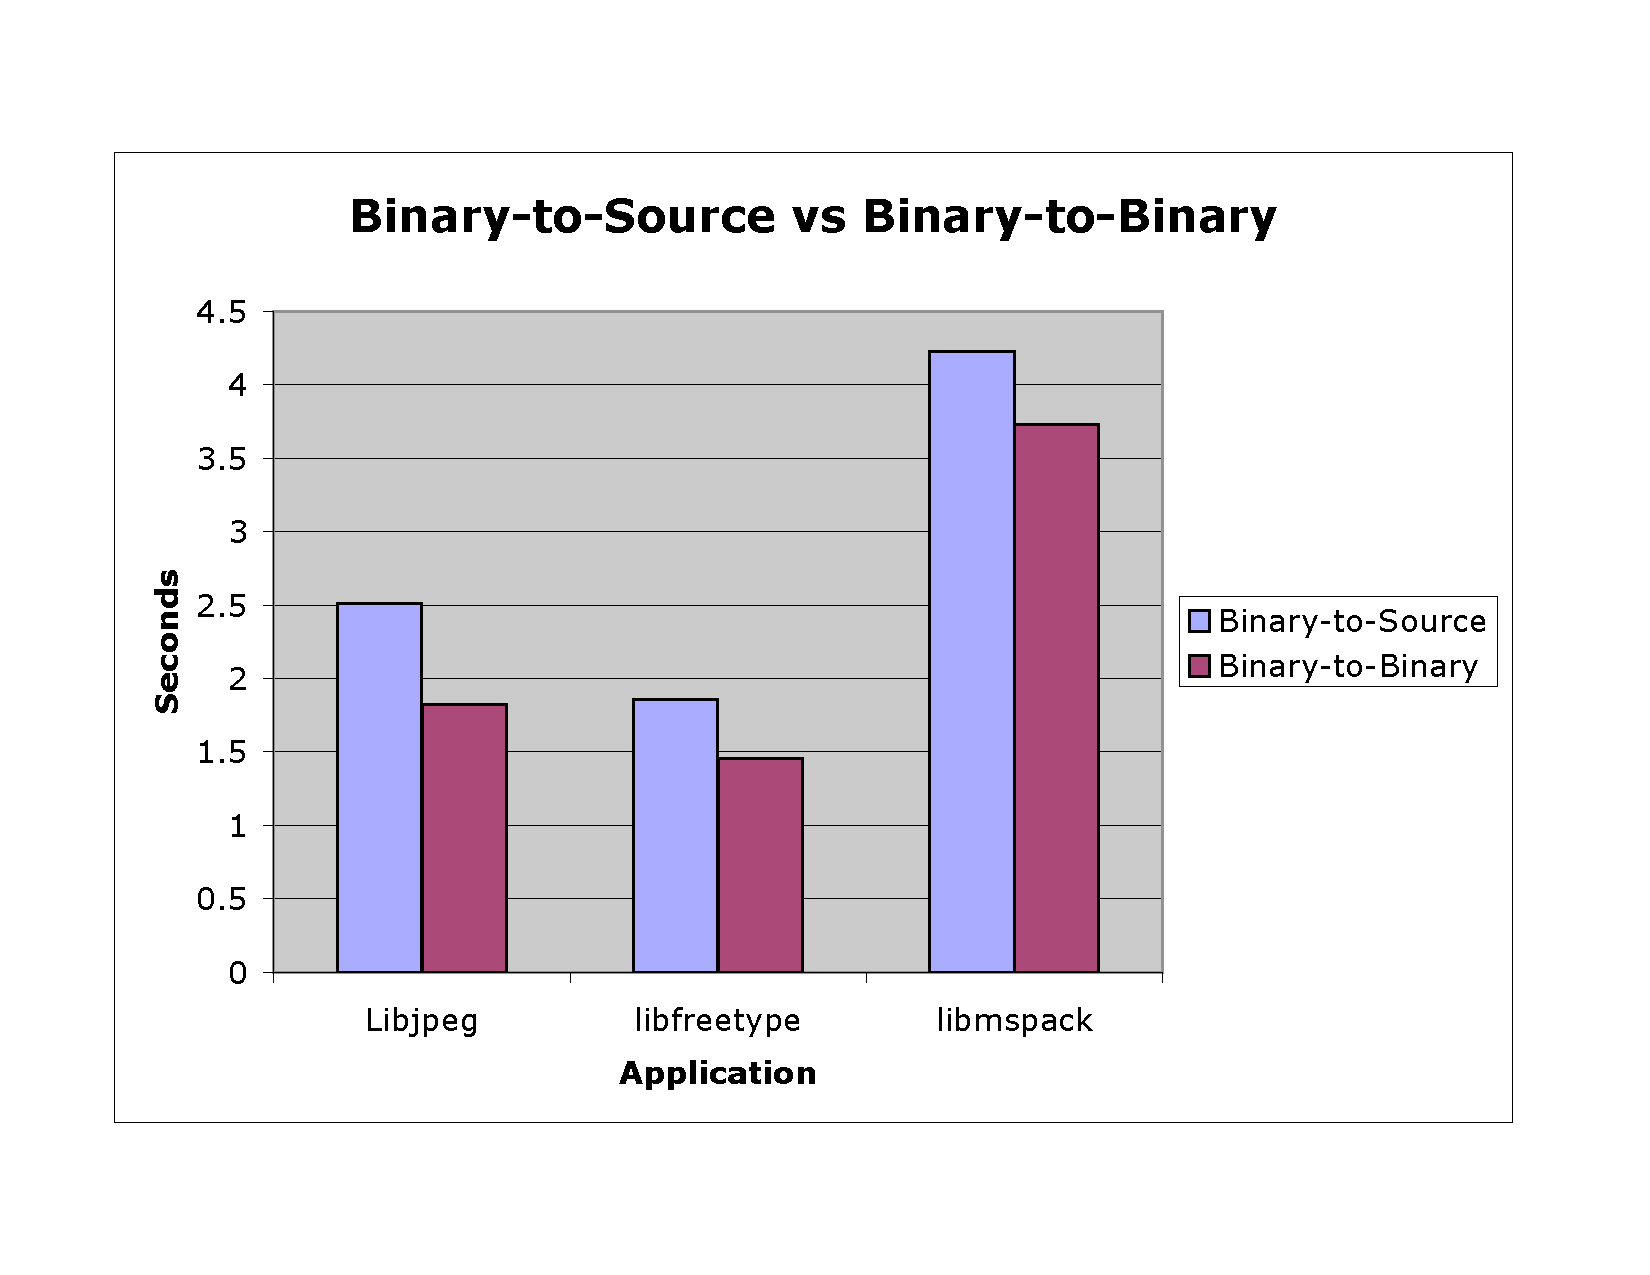
\epsfig{file=chart7,width=3in}

The first optimization gained by direct bytecode generation came from
the use of the JVM {\tt GOTO} instruction.  Despite the fact that the
Java {\it language} does not have a {\tt goto} keyword, the VM does in
fact have a corresponding instruction which is used quite heavily by
{\tt javac}.  NestedVM's binary-to-binary mode exploits this
instruction to avoid emitting inefficient {\tt switch..case}
structures.

Related to the {\tt GOTO} instruction is branch statement
optimization.  When emitting source code, NestedVM translates branches
into Java source code like this:

{\footnotesize\begin{verbatim}
    if (condition) {
        pc = TARGET;
        continue;
    }
\end{verbatim}}

This requires a branch in the JVM {\it regardless} of whether the MIPS
branch is actually taken.  If {\tt condition} is false the JVM has to
jump over the code to set {\tt pc} and go back to the {\tt switch}
statemenmt; if {\tt condition} is true the JVM has to jump to the {\tt
switch} block.  By generating bytecode directly, NestedVM is able to
emit a JVM bytecode branching directly to the address corresponding to
the target of the MIPS branch.  In the case where the branch is not
taken the JVM doesn't branch at all.

A side effect of the previous two optimizations is a solution to the
excess constant pool entries problem.  When jumps are implemented as
{\tt GOTO}s and branches are taken directly, the {\tt pc} field does
not need to be set.  This eliminates a huge number of constant pool
entries.  The {\tt .class} file constant pool size limit is still
present, but it is less likely to be encountered.

Implementation of the MIPS delay slot offers another opportunity for
bytecode-level optimization.  In order to take advantage of
instructions already in the pipeline, the MIPS ISA specifies that the
instruction after a jump or branch is always executed, even if the
jump/branch is taken.  This instruction is referred to as the ``delay
slot\footnote{Newer MIPS CPUs have pipelines that are much larger than
early MIPS CPUs, so they have to discard instructions anyways}.''  The
instruction in the delay slot is actually executed {\it before} the
branch is taken.  To further complicate matters, values from the
register file are loaded {\it before} the delay slot is executed.

Fortunately there is a very elegent solution to this problem which can
be expressed in JVM bytecode.  When a branch instruction is
encountered, the registers needed for the comparison are pushed onto
the stack to prepare for the JVM branch instruction.  Then, {\it
after} the values are on the stack the delay slot instruction is
emitted, followed by the actual JVM branch instruction.  Because the
values were pushed to the stack before the delay slot was executed, any
changes the delay slot made to the registers are not visible to the
branch bytecode.

One final advantage that generating bytecode directly allows is a
reduction in the size of the ultimate {\tt .class} file.  All the
optimizations above lead to more compact bytecode as a beneficial side
effect; in addition, NestedVM performs a few additional optimizations.

When encountering the following {\tt switch} block, both {\tt javac}
and {\tt jikes} generate redundant bytecode.

{\footnotesize\begin{verbatim}
    switch(pc>>>8) {
        case 0x1: run_1(); break;
        case 0x2: run_2(); break
        ...
        case 0x100: run_100(); break;
    }
\end{verbatim}}

The first bytecode in each case arm in the switch statement is {\tt
ALOAD\_0} to prepare for a {\tt INVOKESPECIAL} call.  By simply
lifting this bytecode outside of the {\tt switch} statement, each {\tt
case} arm shrinks by one instruction.

\subsection{Compiler Flags}

Although NestedVM perfectly emulates a MIPS R2000 CPU, its performance
profile is nothing like that of actual silicon.  In particular, {\tt
gcc} makes several optimizations that increase performance on an
actually MIPS CPU but actually decrease the performance of
NestedVM-generated bytecode.  We found the following compiler options
could be used to improve performance:

\begin{itemize}

\item {\tt -falign-functions}

      Normally a function's location in memory has no effect on its
      execution speed.  However, in the NestedVM binary translator,
      the {\tt .text} segment is split on power-of-two boundaries.  If
      a function starts near the end of one of these boundaries, a
      performance critical part of the function winds up spanning two
      Java methods.  Telling {\tt gcc} to align all functions along
      these boundaries decreases the chance of this sort of splitting.

\item {\tt -fno-rename-registers}

      On an actual silicon chip, using additional registers carries no
      performance penalty (as long as none are spilled to the stack).
      However, when generating bytecode, using {\it fewer}
      ``registers'' helps the JVM optimize the machine code it
      generates by simplifying the constraints it needs to deal with.
      Disabling register renaming has this effect.

\item {\tt -fno-schedule-insns}

      Results of MIPS load operations are not available until {\it
      two} instructions after the load.  Without the {\tt
      -fno-schedule-insns} instruction, {\tt gcc} will attempt to
      reorder instructions to do other useful work during this period
      of unavailability.  NestedVM is under no such constraint, so
      removing this reordering typically generates simpler machine
      code.

\item {\tt -mmemcpy}

      Enabling this instruction causes {\tt gcc} to use the system
      {\tt memcpy()} routine instead of generating loads and stores.
      As explained in the next section, the NestedVM runtime
      implements {\tt memcpy()} using {\tt System.arraycopy()}, which
      is substantially more efficient.

\item {\tt -ffunction-sections -fdata-sections}

      These two options are used in conjunction with the {\tt
      --gc-section} linker option, prompting the linker to more
      aggressively prune dead code.

\end{itemize}

The effects of the various optimizations presented in this chapter are
summarized in the table below.

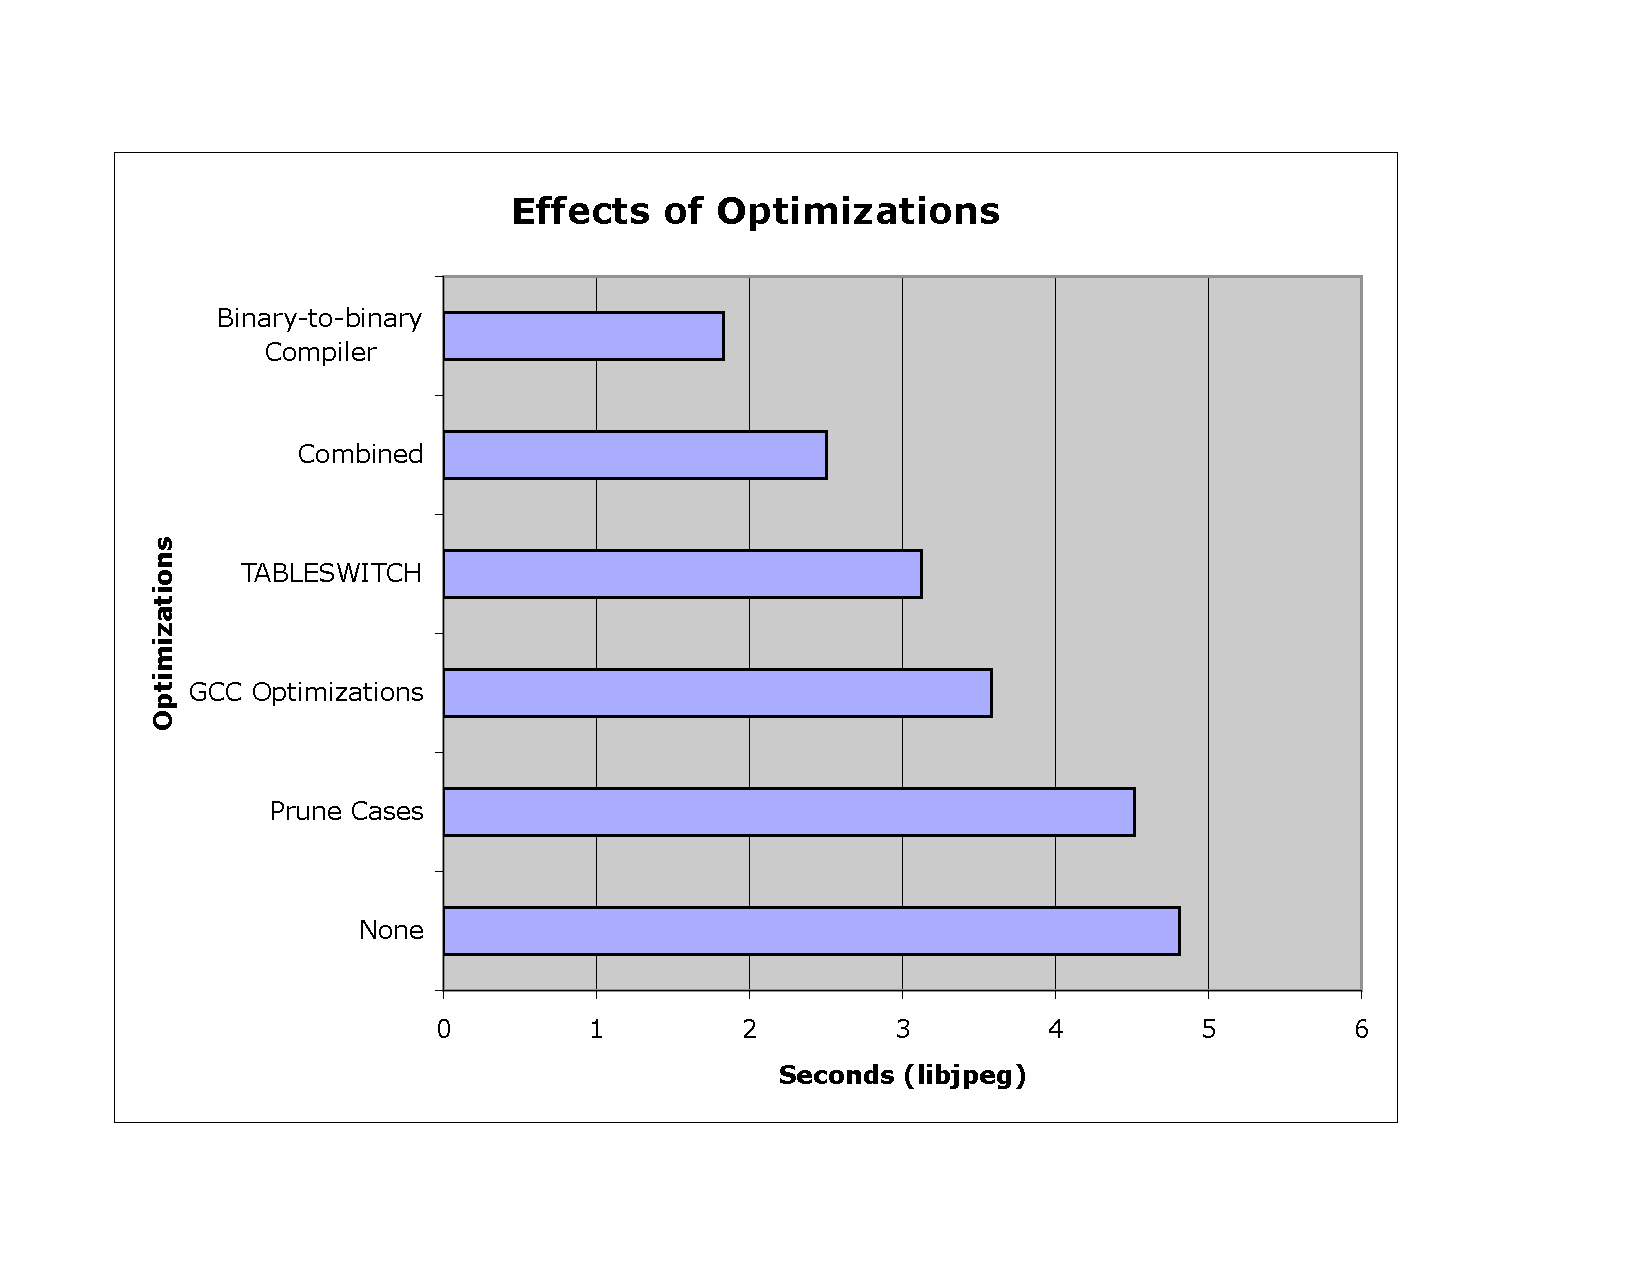
\epsfig{file=chart4,width=3in}

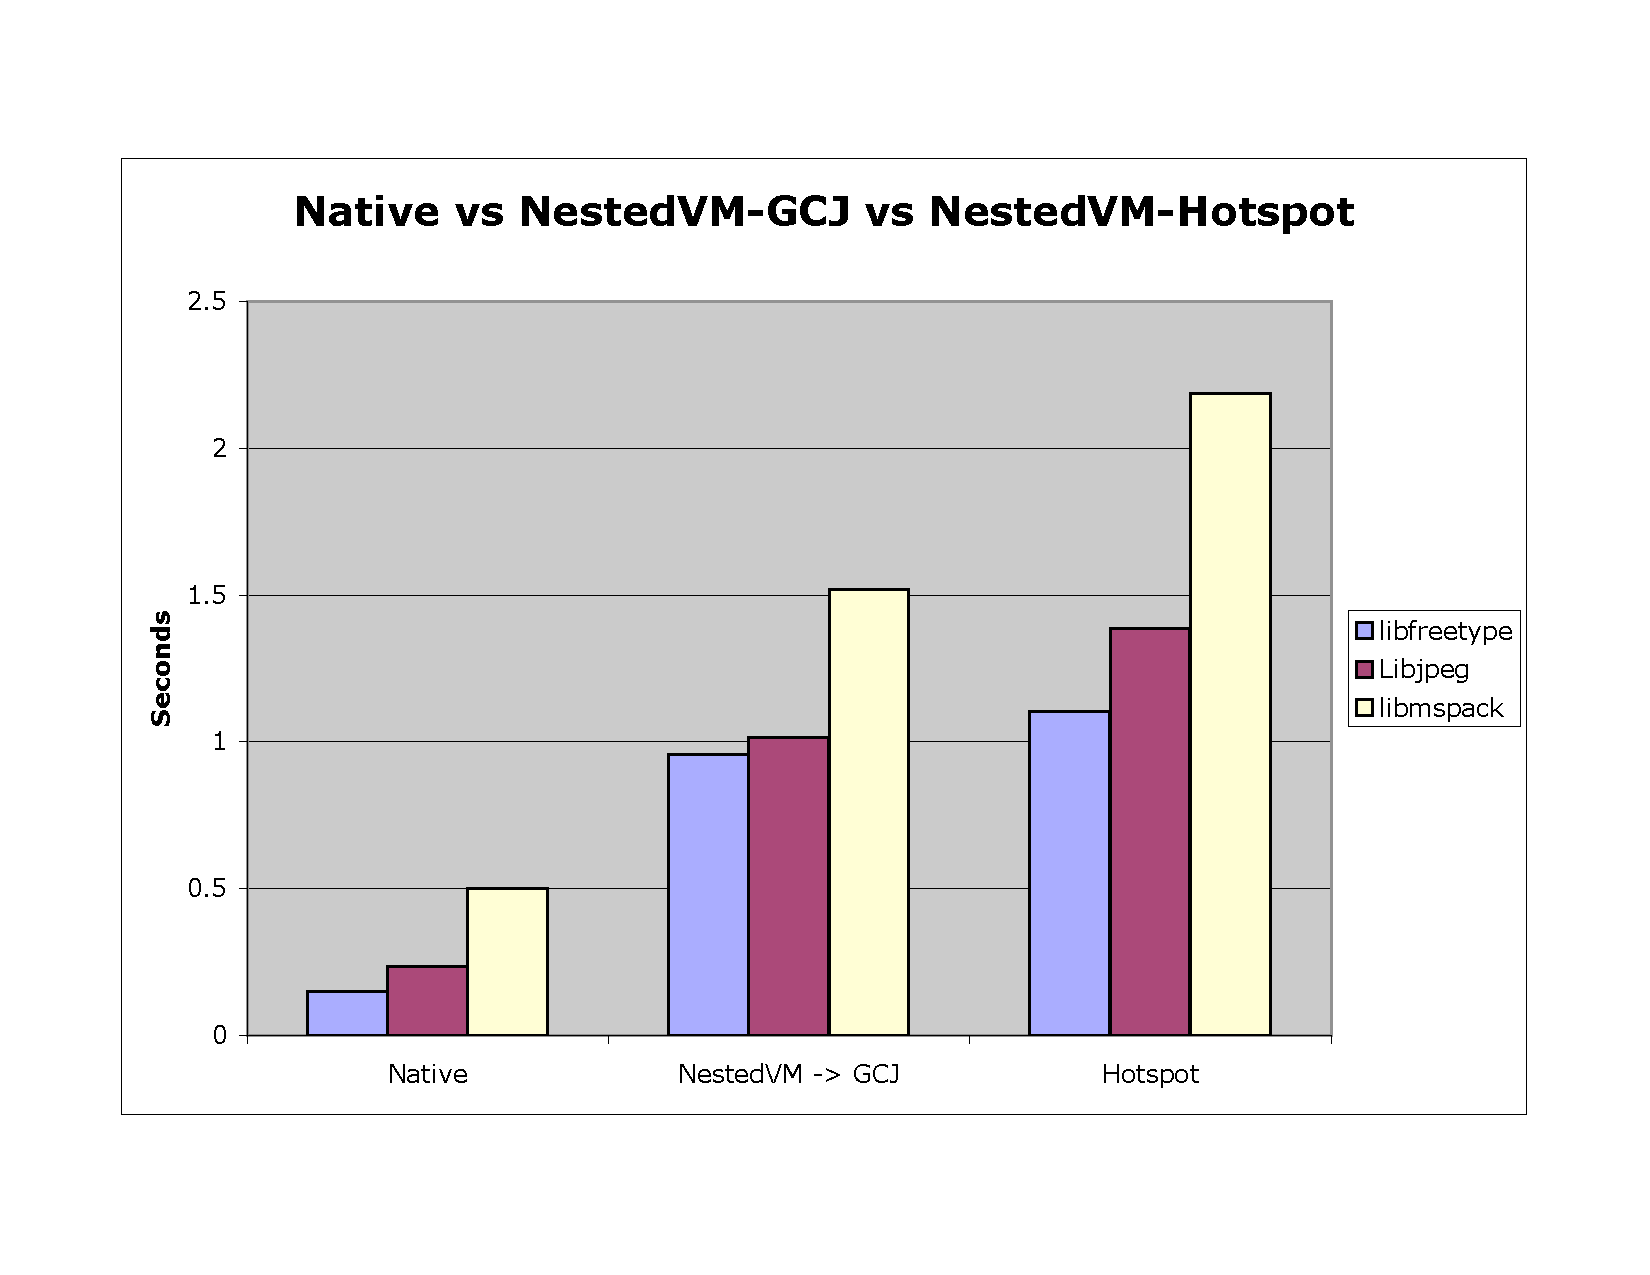
\epsfig{file=chart3,width=3in}


\subsection{FreeType, {\tt libmspack}, and {\tt libjpeg}}

The Ibex Project utilizes three libraries for which no Java-only
equivalent exists.  The first is the FreeType font library, which
parses, hints, and rasterizes TrueType and Postscript fonts with
exceptional quality.  The project also needed an open source JPEG
decompressor; surprisingly, none exist for Java.  While encoders are
plentiful

These three libraries make minimal use of the standard library and OS
services, and are all written in very portable ANSI C code, which made
them easy targets for initial development.

\subsection{The GNU Compiler Collection}

Our next target, {\tt gcc}, was chosen in order to relieve developers
from the time-consuming and complex task of building a compiler
themselves.  The Ibex Project requires a specially configured and
patched version of {\tt gcc} and its ahead-of-time Java compiler ({\tt
gcj}) which is not distributed in binary form.

GCC was the first ``major'' application NestedVM was used on, and
drove the development of most of the system library interface
development; particularly support for {\tt fork()} and {\tt exec()},
which require the NestedVM Runtime to perform binary-to-bytecode
translation on the fly.

GCC also makes extensive use of 64-bit integers ({\tt long long}),
which -- for performance reasons -- are typically manipulated using
nonobvious instruction sequences on the 32-bit MIPS architecture.
Dealing with these operations uncovered a number of bugs in the
translator.

Despite our original goal, we have not yet been able to translate the
{\tt C++} or Java front-ends, as the resulting binary produces a
trampoline which exceeds the maximum size of a single method.  Future
work will explore a multi-level trampoline to address this issue.



\subsection{\TeX and LINPACK}

In order to distinguish NestedVM from other single-language
translators for the JVM, we undertook the task of translating \TeX 89
(written in Pascal) and the Fortran source code for LINPACK into Java
bytecodes.

Although actually producing the initial MIPS binaries from the \TeX\
source code turned out to be an exceptionally tedious and frustrating
task, the resulting binary translated and executed perfectly on the
first run, as did LINPACK.  Our reward for this effort was typesetting
our presentation of NestedVM using NestedVM itself.  We have also had
initial successes running \TeX\ in a Java Applet, and intend to
produce a {\tt jar} for embedding \TeX\ code (``\TeX lets'') in web
pages without the use of a post-processing tool.

The LINPACK benchmark called our attention to Java's lack of an API
for checking the ``cpu time'' of a process.  Unfortunately we had to
substitute wall-clock time on an otherwise-quiescent machine as an
approximation.



\section{The NestedVM Runtime}

In addition to binary-to-source and binary-to-binary translation,
NestedVM also includes a MIPS binary interpreter.  All three
translation approaches expose the same API to both the translated
binary and the surrounding VM (including peer Java code).

The NestedVM Runtime (various subclasses of {\tt
org.ibex.nestedvm.Runtime}) fill the role of an OS Kernel.
Communication between MIPS code and the outside world is via the MIPS
{\tt SYSCALL} instruction, just as the {\tt libc}-kernel interface is
on real MIPS implementations.

Two implemenations of the runtime are offered; a simple runtime with
the minimum support required to comply with ANSI C, and a more
sophisticated runtime which emulates a large portion of the POSIX API.

\subsection{The ANSI C Runtime}

The ANSI C runtime offers typical file I/O operations including {\tt
open()}, {\tt close()}, {\tt read()}, {\tt write()}, and {\tt seek()}.
File descriptors are implemented much as they are in OS kernels; a
table of open files is maintained and descriptors act as an index into
that table.  Each file is represented as a Java {\tt RandomAccessFile}
in order to match the semantics of {\tt seek()}.

Process-level memory management is done through the {\tt sbrk()}
system call, which extends the process heap by adding more pages to
the memory page table.  Fast memory clear and copy operations can be
performed with {\tt memset()} and {\tt memcpy()}, which invoke the
Java {\tt System.arraycopy()} method, which is generally much faster
than a {\tt for()} loop.

The {\tt exit()} call records the exit status, marks the VM instance
as terminated and halts execution.  The {\tt pause()} syscall
implements a crude form of Java-MIPS communication by returning
control to the Java code which spawned the MIPS process.

\subsection{The Unix Runtime}

The Unix runtime extends the simple ANSI file I/O model to include a
single-root filesystem, and device nodes, as well as {\tt fcntl()}
APIs to manipulate these.  Device nodes are generally simulated by
mapping reads, writes, and {\tt fcntl()}s on the device to the
appropriate Java API.

MIPS processes can ``mount'' other filesystems within the virtual
filesystem made visible to the MIPS process.  Each filesystem is
implemented by a Java class, which could, for example, offer access to
the host filesystem (including {\tt state()}, {\tt lstat()}, {\tt
mkdir}, and {\tt unlink()}, and {\tt getdents()}), the contents of a
zip archive, or even a remote HTTP server.

MIPS processes can also spawn subprocesses using the {\tt fork()} and
{\tt exec()} calls, which create new Java threads to run the process.
The {\tt fork()} call -- which is supposed to duplicate the memory
image of a process -- is implemented in an elegant manner by calling
the Java {\tt clone()} method (deep copy) on the VM object itself.
Copy-on-write is not currently implemented.  The new instance is added
to a static process table to facilitate interprocess communication.

The {\tt waitpid()} API allows a parent process to block pending the
completion of a child process, which is done quite easily with the
Java {\tt wait()} method.

The {\tt exec()} method actually loads a MIPS binary image from the
filesystem, feeds it to the MIPS-to-bytecode translator, and then
loads the resulting bytecode on the fly using {\tt
ClassLoader.loadBytes()}.  The {\tt pipe()} system call permits
parent-to-child IPC just as on a normal Unix system.

Simple networking support is provided by the {\tt opensocket()}, {\tt
listensocket()}, and {\tt accept()} methods, which are not currently
compatible with the usual Berkeley sockets API.


\subsection{Security Concerns}

RuntimeExceptions don't escape, they care caught and turned into
checked exceptions filesystem access does though security manager
(NestedVM Runtime.SecurityManager, and the JVM's)


\subsection{Threading}

The NestedVM runtime currently does not support threading.  Providing
robust support for ``true threads'', whereby each MIPS thread maps to
a Java thread is probably not possible as the Java Memory Model
[CITE], since all MIPS memory is stored in a set of {\tt int[]}'s and
the Java Memory Model does not permit varying treatment or coherency
policies at the granularity of a single array element.

While this presents a major barrier for applications that use
sophisticated locking schemes (such as {\it hash synchronization})
which depend on atomic memory operations, it is probably possible to
apply this threading model to ``well behaved'' multithreaded
applications which depend only on OS-provided semaphores and mutexes
for synchronization.

Complex synchronization and incorrectly synchronized applications can
be supported by implementing a variant of {\it user threads} within a
single Java thread by providing a timer interrupt (via a Java
asynchronous exception).  Unfortunately this requires that the
compiled binary be able to restart from any arbitrary instruction
address, which would require a {\tt case} statement for every
instruction (rather than every jump target), which would degrade
performance and increase the size of the resulting class file.


\section{Conclusion}

\subsection{Theoretical Limitations}

Theoretical limitations: threads, reading from code, self-modifying
code, COW?

\subsection{Future Directions}

Although we have only implemented it for the Java Virtual Machine, our
technique generalizes to other safe bytecode architectures.  In
particular we would like to demonstrate this generality by retargeting
the translator to the Microsoft Intermediate Language \cite{msil}.

Additionally, we would like to explore other uses for dynamic loading
of translated MIPS binaries by combining NestedVM (which itself is
written in Java) and the {\tt ClassLoader.fromBytes()} mechanism.

\subsection{Availability}

NestedVM is available under an open source license, and can be
obtained from
\begin{verbatim}
    http://nestedvm.ibex.org
\end{verbatim}

\appendix
\section{Appendix: Testing Methodology}

All times are measured in seconds. These were all run on a dual 1Ghz
Macintosh G4 running Apple's latest JVM (Sun HotSpot JDK 1.4.1). Each
test was run 8 times within a single VM. The highest and lowest times
were removed and the remaining 6 were averaged.  In each case only the
first run differed significantly from the rest.

The {\tt libjpeg} test consisted of decoding a 1280x1024 jpeg and
writing a tga.  The {\tt mspack} test consisted of extracting all
members from {\tt arial32.exe}, {\tt comic32.exe}, {\tt times32.exe},
and {\tt verdan32.exe}. The {\tt libfreetype} test consisted of
rendering ASCII characters 32-127 of {\tt Comic.TTF} at sizes from 8
to 48 incrementing by 4 for a total of 950 glyphs.

\bibliography{nestedvm}

\end{document}

